\section{Forging Optimization Control}
% 本节提出一种基于安全离线强化学习的锻造优化控制训练框架，通过离线训练使智能体根据锻件初始温度场，在满足损伤约束的前提下，直接生成完整锻造过程的最优速度曲线，实现开环规划，具体如图\ref{fig:control-1}所示。

% 为求解该问题，将过程建模为上下文赌博机模型\cite{bouneffouf2020survey}，其元组 $(\mathcal{S}, \mathcal{A}, \mathcal{R}, \mathcal{C})$ 定义如下：

% \textbf{状态空间$\mathcal{S}$}：观测状态$\mathbf S\in\mathcal{S}$为锻件中$N$个微元的位置和温度,其中每个微元表示为$\mathbf{s}_i=\{x_i, y_i, z_i, T_i\}$，完整观测状态$\mathbf{S}\in\mathbb{R}^{N*4}$。

% \textbf{动作空间$\mathcal{A}$}：锻造速度决策$\mathbf a\in \mathcal{A}$采用四个参数$\mathbf a =[v_0,v_1,t_0,t_1]$进行表示，其与曲线的映射关系见章节\ref{sec:speed}。

% \textbf{奖励$R$}：定义为锻造效率与锻件内部应力的加权组合
% \begin{equation}
%   R = \underbrace{w_1 \cdot \exp(-time)}_{\text{time\_reward}} - \underbrace{w_2  \cdot \exp(stress)}_{\text{stress\_penalty}}
% \end{equation}
% 作为奖励,其中$\text{stress\_penalty}$奖励较小应力，$\text{time\_reward}$奖励生产效率，$w_i$为权重系数。

% \textbf{安全约束$\mathcal{C}$}：基于Normalized Cockcroft \& Latham断裂准则计算损伤值:
% \begin{equation}
% D(t) = \int_{0}^{t} \frac{\max(\sigma_1(\tau), 0)}{\bar{\sigma}(\tau)} \dot{\bar{\varepsilon}}(\tau) d\tau
% \end{equation}
% 损伤累积值$D(t)$来表征$C$，它是材料在变形过程中，其最大拉应力与等效应力之比乘上当前应变随时间的积分值，
% 当$C$超过材料临界损伤$C_0$时视为断裂。

% 本研究的目标是从有限元仿真生成的静态数据集 $\mathcal{B} = \{ (s_i, a_i, r_i, c_i) \}_{i=1}^{N}$中学习最优策略网络 $\pi^{*}$,在满足成本约束的前提下最大化奖励。所有策略的训练与评估均基于数据集 $\mathcal{B}$离线完成，无需与实际锻压设备交互。
This section proposes a safe offline reinforcement learning framework
for forging optimization. The agent is trained offline to generate an
optimal speed profile based on the initial temperature field, satisfying
damage constraints for open-loop planning (Fig. \ref{fig:control-1}).

The problem is formulated as a contextual bandit model
\cite{bouneffouf2020survey}, defined by the tuple
$(\mathcal{S}, \mathcal{A}, \mathcal{R}, \mathcal{C})$:

\textbf{State space $\mathcal{S}$}: The observation state
$\mathbf{S} \in \mathcal{S}$ comprises the positions and temperatures of
$N$ micro-elements in the workpiece,
$\mathbf{s}_i = \{x_i, y_i, z_i, T_i\}$, forming
$\mathbf{S} \in \mathbb{R}^{N \times 4}$.

\textbf{Action space $\mathcal{A}$}: The forging speed decision
$\mathbf{a} \in \mathcal{A}$ is parameterized as
$\mathbf{a} = [v_0, v_1, t_0, t_1]$, mapping to a curve as defined in
Section \ref{sec:speed}.

\textbf{Reward $\mathcal{R}$}: A weighted combination of efficiency and
internal stress:
\begin{equation}
R = \underbrace{w_1 \cdot \exp(-\text{time})}_{\text{time\_reward}} - \underbrace{w_2 \cdot \exp(\text{stress})}_{\text{stress\_penalty}}
\end{equation}
where the time reward promotes productivity and the stress penalty
discourages high stress.

\textbf{Cost $\mathcal{C}$}: Damage is evaluated via the normalized
Cockcroft \& Latham criterion:
\begin{equation}
D(t) = \int_{0}^{t} \frac{\max(\sigma_1(\tau), 0)}{\bar{\sigma}(\tau)} \dot{\bar{\varepsilon}}(\tau) d\tau
\end{equation}
Cost $C$ is the cumulative damage $D(t)$. Fracture occurs when $C$
exceeds the critical value $C_0$.

The objective is to learn an optimal policy $\pi^*$ from a static
dataset $\mathcal{B} = \{ (s_i, a_i, r_i, c_i) \}_{i=1}^{N}$ generated
by finite element simulations, maximizing reward while satisfying the
cost constraint. All policy training and evaluation is performed offline
on $\mathcal{B}$, with no interaction with the physical forging
equipment.

\begin{figure}[htbp]
\centerline{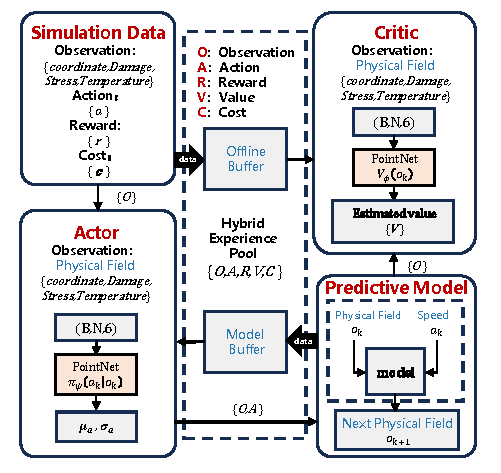
\includegraphics[width=\linewidth]{control-1.pdf}}
\caption{Training architecture of policy network .}
\label{fig:control-1}
\end{figure}
% 决策网络基于 PointNet\cite{qi2017pointnet} 架构构建，实现了温度场到速度曲线参数的映射。
% 决策网络训练使用混合经验池，包含当前策略生成的交互数据与历史仿真数据。为实现带约束的策略优化，可引入拉格朗日松弛法将原约束问题转化为无约束形式。具体地，构造拉格朗日函数：
% \begin{equation}
% L(\psi, \lambda) = \mathbb{E}_{ p_{\psi}} \left[ \ln p_{\psi}(a|
% s) \cdot A(s,a) \right]
% \end{equation}
% 其中,优势函数为：
% \begin{equation}
% A(s,a) = R - V(s) - \lambda \cdot \mathrm{relu}(c - c_0)
% \end{equation}
% V(s)是通过蒙特卡洛采样估计的期望奖励。对于给定的初始状态$s$，从当前策略网络 $\pi_{\psi}(a|s)$中蒙特卡洛采样 $N$个动作 $\{a_{j} \}_{j=1}^N$，每个动作 $a_j$对应一条速度曲线。将这些动作输入代理模型，预测场量状态，计算每个动作的奖励 $R(a_j)$，然后取平均值作为价值估计：
% \begin{equation}
% V(s) = \mathbb{E}_{a \sim \pi_{\psi}(\cdot|s)} [R(s, a)] \approx \frac{1}{N} \sum_{j=1}^{N} R(s, a_j)
% \end{equation}

% 为鼓励策略探索并防止过早收敛，在优化目标中加入熵正则化项：
% \begin{equation}
% J(\psi, \lambda) = L(\psi, \lambda) + \eta H[a|s)]
% \end{equation}
% 该优化问题通过对偶梯度上升法求解：在每一步迭代中，首先固定对偶变量 $\lambda$，通过梯度上升更新策略参数 $\psi$ 以最大化拉格朗日函数；然后固定策略参数 $\psi$，根据约束违反程度更新对偶变量 $\lambda$。对偶变量的更新规则为：
% \begin{equation}
% \lambda \leftarrow \max(0, \lambda + \alpha_{\lambda} (c - c_0))
% \end{equation}
% 当损伤值 $c$ 超过阈值 $c_0$ 时，对偶变量 $\lambda$ 增加以加强约束惩罚，反之则减小惩罚力度。

The policy network, built on the PointNet architecture
\cite{qi2017pointnet}, maps the temperature field to speed profile
parameters. It is trained using a hybrid experience replay buffer
containing data from both the current policy and historical simulations.

Constrained policy optimization is achieved via Lagrangian relaxation,
transforming the problem into an unconstrained form. The Lagrangian is
defined as:
\begin{equation}
L(\psi, \lambda) = \mathbb{E}_{p_{\psi}} \left[ \ln p_{\psi}(a|s) \cdot A(s,a) \right]
\end{equation}
with the advantage function:
\begin{equation}
A(s,a) = R - V(s) - \lambda \cdot \mathrm{relu}(c - c_0)
\end{equation}
Here, $V(s)$ is the expected reward estimated via Monte Carlo sampling.
Given an initial state $s$, $N$ actions $\{a_j\}_{j=1}^N$ are sampled
from the current policy $\pi_{\psi}(a|s)$. Each action $a_j$ corresponds
to a speed profile. The surrogate model predicts the resulting field
states, and the value is estimated as:
\begin{equation}
V(s) \approx \frac{1}{N} \sum_{j=1}^{N} R(s, a_j)
\end{equation}

To encourage exploration and prevent premature convergence, an entropy
regularization term is added:
\begin{equation}
J(\psi, \lambda) = L(\psi, \lambda) + \eta H[a|s]
\end{equation}
The optimization is solved using dual gradient ascent. In each
iteration, the policy parameters $\psi$ are updated to maximize $J$ with
fixed $\lambda$, and then the dual variable is updated based on
constraint violation:
\begin{equation}
\lambda \leftarrow \max(0, \lambda + \alpha_{\lambda} (c - c_0))
\end{equation}
This increases the penalty when the damage $c$ exceeds the threshold
$c_0$, and decreases it otherwise.
